\documentclass[11pt]{article}

\usepackage[margin=0.85in]{geometry}
\usepackage{amsmath, amssymb}
\usepackage{graphicx}
\usepackage{booktabs}
\usepackage{hyperref}
\usepackage{xcolor}
\usepackage{enumitem}
\usepackage{float}
\usepackage{caption}
\usepackage{subcaption}
\usepackage{listings}

\hypersetup{
  colorlinks=true,
  linkcolor=blue,
  urlcolor=blue,
  citecolor=blue
}

\lstset{
  basicstyle=\ttfamily\small,
  breaklines=true,
  frame=single,
  columns=fullflexible,
  keepspaces=true,
  showstringspaces=false
}

\title{Numerical Modeling of RF Ion-Trap Geometries in \texttt{multipole\_table\_replication.ipynb}}
\author{Generated Report}
\date{\today}

\begin{document}
\maketitle

\begin{abstract}
This document explains the methods, mathematics, physics, and code structure used
in \texttt{multipole\_table\_replication.ipynb}. The notebook builds several
two-dimensional ion-trap electrode geometries, solves the electrostatic
Laplace problem for the normalized RF potential, computes the RF
pseudopotential for a trapped \({}^{9}\mathrm{Be}^{+}\) ion, extracts
multipole ratios, validates the numerical solution, and produces geometry,
field, pseudopotential, profile, and trap-depth plots. The notebook includes the
original traps labeled (a)--(h), whiteboard blade-trap variants, an angled
five-electrode sweep, and a sketch-based surface trap sweep. The goal is to
compare how electrode geometry changes the shape and depth of the RF
pseudopotential.
\end{abstract}

\tableofcontents
\newpage

\section{Purpose of the Notebook}

The notebook is a computational experiment for comparing candidate RF ion-trap
cross sections. It does not attempt a full three-dimensional trap simulation.
Instead, it models a two-dimensional cross section in the \(x\)-\(y\) plane and
assumes the electrodes are translationally invariant in the third direction.
This is a common first approximation for long linear traps or surface-electrode
cross sections when the main question is how electrode placement changes the
local RF curvature, pseudopotential confinement, and trap depth.

The notebook has four main goals:
\begin{enumerate}[label=\arabic*.]
  \item Reproduce and compare several named geometries, labeled (a)--(h).
  \item Solve the Laplace equation for each electrode layout using fixed
        Dirichlet electrode voltages.
  \item Convert the RF electric field into a ponderomotive pseudopotential for
        \({}^{9}\mathrm{Be}^{+}\).
  \item Plot the RF potential, pseudopotential, line-cut trap depth, and
        geometry-dependent depth summaries.
\end{enumerate}

The notebook treats RF electrodes as fixed at a normalized voltage of \(+1\) in
the Laplace solve. Some outer or ground-like electrodes are assigned \(0\) V or
\(-1\) V depending on the geometry being studied. The physical RF amplitude is
applied later when computing the pseudopotential. In the current notebook, the
important physical constants are
\[
  m = 9.0121831\,u = 1.4965\times 10^{-26}\ \mathrm{kg},
\]
\[
  q = e = 1.602176634\times 10^{-19}\ \mathrm{C},
\]
\[
  V_{\mathrm{RF}} = 500\ \mathrm{V}, \qquad
  \Omega_{\mathrm{RF}} = 2\pi(30\ \mathrm{MHz}).
\]
These constants appear in the first code cell as \texttt{ION\_MASS},
\texttt{Q\_E}, \texttt{V\_RF\_AMP}, and \texttt{OMEGA\_RF}.

\subsection{Main Outputs}

For each simulated trap, the notebook usually creates:
\begin{itemize}
  \item a two-panel main plot containing \(\phi_{\mathrm{rf}}\) and shifted
        pseudopotential \(\Phi_{\mathrm{ps}}-\Phi_{\min}\);
  \item a pseudopotential line-cut/profile plot with an estimated depth marker;
  \item multipole ratio tables for \(\phi_{\mathrm{rf}}\) and, where
        meaningful, for \(\Phi_{\mathrm{ps}}\);
  \item CSV summary files for later comparison; and
  \item validation output checking the numerical solution.
\end{itemize}

\newpage

\section{Geometry Representation}

Each trap is represented as a list of electrode dictionaries. A typical
electrode dictionary contains
\begin{lstlisting}[language=Python]
{
    'cx': center_x,
    'cy': center_y,
    'w': width,
    'h': height,
    'V': voltage,
    'label': 'RF' or 'GND',
    'poly': optional_polygon_vertices
}
\end{lstlisting}
Rectangular electrodes can be represented by \(\texttt{cx}\), \(\texttt{cy}\),
\(\texttt{w}\), and \(\texttt{h}\). More general tilted or beveled electrodes
are represented by \(\texttt{poly}\), a list of polygon vertices. The same
solver function supports both cases by using \texttt{polygon\_mask} for polygon
electrodes and a rectangular mask otherwise.

\subsection{Original Traps (a)--(h)}

The notebook defines geometry builders for traps (a)--(h):
\begin{itemize}
  \item \texttt{trap\_a\_2layer}: four trapezoidal electrodes around a central
        open region.
  \item \texttt{trap\_b\_balanced}: a related four-electrode balanced geometry.
  \item \texttt{trap\_c\_3layer}: a six-electrode pointed geometry.
  \item \texttt{trap\_d\_algaas}: a very thin vertical stack.
  \item \texttt{trap\_e\_inplane4}: a simple four-wire in-plane geometry.
  \item \texttt{trap\_f\_4wire\_surface}: a surface-electrode style
        four-wire trap.
  \item \texttt{trap\_g\_5wire\_symm}: a symmetric five-wire surface trap.
  \item \texttt{trap\_h\_5wire\_asymm}: an asymmetric five-wire surface trap.
\end{itemize}

For the surface-style traps, the ion/RF-null reference point is taken to be
\((0,0)\), while the electrodes are placed below the ion plane. For example,
several surface geometries use an electrode plane near \(y=-40\ \mu\mathrm{m}\).
This convention lets the same solver and analysis routines be used across many
geometries.

\subsection{Sketch-Based Geometry Generator}

The newer sketch-based section creates five surface-electrode geometries at
\[
  \theta = 0^\circ,\ 22.5^\circ,\ 45^\circ,\ 67.5^\circ,\ 90^\circ .
\]
The functions
\texttt{create\_rotated\_rectangle},
\texttt{create\_horizontal\_rectangle}, and
\texttt{generate\_trap\_geometry}
construct the electrode polygons directly from centerline geometry.

For an angled RF segment starting at point \(\mathbf{s}\), length \(L\),
thickness \(t\), and angle \(\theta\), the unit tangent and normal are
\[
  \mathbf{u} = (\cos\theta,\sin\theta), \qquad
  \mathbf{n} = (-\sin\theta,\cos\theta).
\]
The segment endpoint is
\[
  \mathbf{e} = \mathbf{s} + L\mathbf{u},
\]
and the rectangle vertices are
\[
  \mathbf{s}-\frac{t}{2}\mathbf{n},\quad
  \mathbf{e}-\frac{t}{2}\mathbf{n},\quad
  \mathbf{e}+\frac{t}{2}\mathbf{n},\quad
  \mathbf{s}+\frac{t}{2}\mathbf{n}.
\]
The outer RF pads are then placed from the endpoint \(\mathbf{e}\) of the
angled RF segment. This is important: the outer pad location is not manually
guessed for each angle. Instead, the endpoint is computed and used as the pad
start point, so the pad remains connected to the slanted RF segment as
\(\theta\) changes.

\begin{figure}[H]
  \centering
  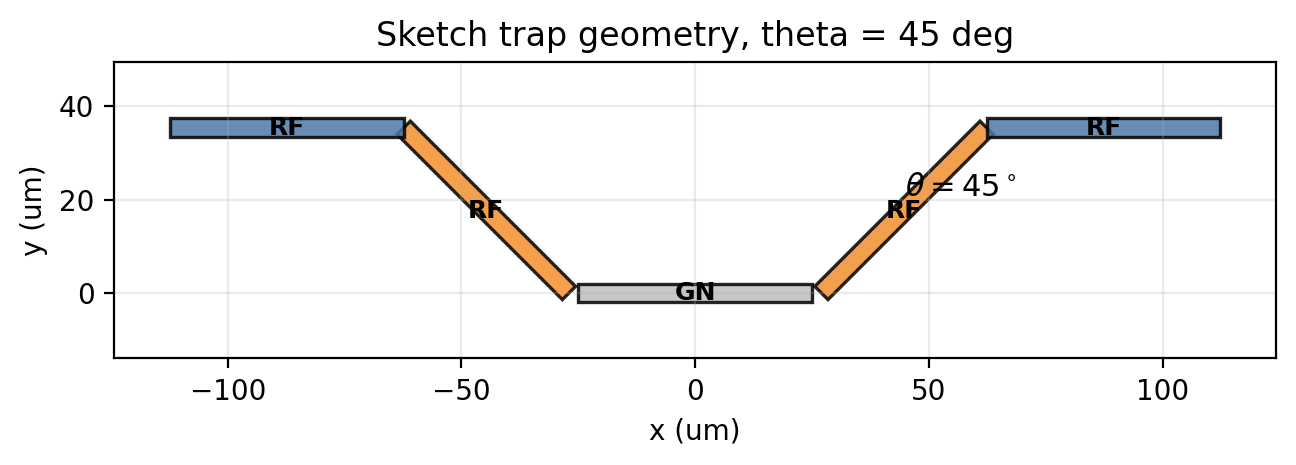
\includegraphics[width=0.82\linewidth]{pngs/sketch_trap_theta_45p0deg.png}
  \caption{Example generated sketch geometry at \(\theta=45^\circ\). The
  central ground electrode is labeled GN, and all RF electrodes are labeled RF.
  The outer pads are horizontal and are built from the endpoints of the angled
  RF segments.}
\end{figure}

\newpage

\section{The Electrostatic Boundary-Value Problem}

The core physics calculation starts with an electrostatic boundary-value
problem. In charge-free vacuum between electrodes, the potential satisfies
Laplace's equation:
\[
  \nabla^2 \phi_{\mathrm{rf}}(x,y) = 0.
\]
The notebook solves this equation on a uniform rectangular grid. The boundary
conditions are:
\begin{itemize}
  \item RF electrode pixels are fixed to their normalized voltage, typically
        \(+1\).
  \item Ground electrodes are fixed to \(0\), unless a studied geometry assigns
        an outer electrode to \(-1\).
  \item The outer computational domain boundary is grounded.
  \item All non-electrode interior pixels satisfy the discrete Laplace equation.
\end{itemize}

\subsection{Finite-Difference Discretization}

For uniform grid spacings \(\Delta x\) and \(\Delta y\), the second-order
finite-difference approximation is
\[
  \nabla^2 \phi_{i,j}
  \approx
  \frac{\phi_{i+1,j}-2\phi_{i,j}+\phi_{i-1,j}}{\Delta x^2}
  +
  \frac{\phi_{i,j+1}-2\phi_{i,j}+\phi_{i,j-1}}{\Delta y^2}.
\]
Most grids in the notebook use square pixels, so \(\Delta x=\Delta y\), and the
interior stencil can be written as
\[
  \phi_{i,j}
  =
  \frac{1}{4}
  \left(
    \phi_{i+1,j}+\phi_{i-1,j}+\phi_{i,j+1}+\phi_{i,j-1}
  \right).
\]

The function \texttt{solve\_laplace} assembles this finite-difference system as
a sparse linear system,
\[
  A\mathbf{v} = \mathbf{b}.
\]
Each grid point contributes one row. For fixed electrode or domain-boundary
pixels, the row enforces
\[
  v_k = V_{\mathrm{fixed}}.
\]
For interior pixels, the row enforces the five-point Laplace stencil. The
notebook then solves the sparse system using SciPy's direct sparse solver
\texttt{spsolve}.

\subsection{Electrode Masks}

The first step in \texttt{solve\_laplace} is to convert every electrode into a
boolean mask on the numerical grid. The code calls
\texttt{electrode\_mask}, which either:
\begin{itemize}
  \item evaluates a polygon mask for tilted/beveled electrodes, or
  \item evaluates an axis-aligned rectangle mask for simple rectangular
        electrodes.
\end{itemize}
The mask determines which grid points are Dirichlet electrode pixels. This is
also why the sketch-trap simulation uses a tiny solver-only contact gap between
different-voltage touching electrodes. In the physical sketch, the electrodes
touch. On a finite-difference grid, however, two different voltages cannot be
assigned to the same pixel. The small contact gap preserves a well-defined
masking problem while keeping the visual geometry endpoint-based.

\newpage

\section{RF Pseudopotential Physics}

An ion in an RF trap experiences a rapidly oscillating electric field. If the
RF drive is fast compared with the secular motion, the ion motion can be
separated into a fast micromotion and a slower secular motion. The slow motion
is governed approximately by the ponderomotive pseudopotential.

Let the time-dependent RF potential be
\[
  \phi(x,y,t) = V_{\mathrm{RF}}\phi_{\mathrm{rf}}(x,y)\cos(\Omega t),
\]
where \(\phi_{\mathrm{rf}}\) is the dimensionless Laplace solution with RF
electrodes set to \(1\) V. The electric field amplitude is
\[
  \mathbf{E}_{0}(x,y)
  =
  -V_{\mathrm{RF}}\nabla\phi_{\mathrm{rf}}(x,y).
\]
The standard pseudopotential energy is
\[
  U_{\mathrm{ps}}(x,y)
  =
  \frac{q^2}{4m\Omega^2}
  |\mathbf{E}_{0}(x,y)|^2.
\]
The notebook reports an equivalent pseudopotential in volts by dividing the
energy by \(q\):
\[
  \Phi_{\mathrm{ps}}(x,y)
  =
  \frac{U_{\mathrm{ps}}}{q}
  =
  \frac{q}{4m\Omega^2}
  \left(V_{\mathrm{RF}}^2|\nabla\phi_{\mathrm{rf}}(x,y)|^2\right).
\]
This is exactly the expression used in the function \texttt{pseudopotential}:
\[
  \Phi_{\mathrm{ps}}
  =
  \frac{q}{4m\Omega^2}
  \left[
    V_{\mathrm{RF}}^2
    \left(
      \left(\frac{\partial\phi_{\mathrm{rf}}}{\partial x}\right)^2
      +
      \left(\frac{\partial\phi_{\mathrm{rf}}}{\partial y}\right)^2
    \right)
  \right].
\]
The code converts the grid spacing from micrometers to meters before taking the
gradient. This matters because \(\nabla\phi_{\mathrm{rf}}\) must have units of
\(\mathrm{m}^{-1}\), so that \(V_{\mathrm{RF}}\nabla\phi_{\mathrm{rf}}\) has
units of \(\mathrm{V/m}\).

\subsection{Why the Pseudopotential is Shifted}

The notebook often plots
\[
  \Phi_{\mathrm{ps}}(x,y) - \Phi_{\min},
\]
where \(\Phi_{\min}\) is the local pseudopotential minimum near the RF null.
This shift is not a change in the physics. It simply makes the plots easier to
read because trap depth and confinement are controlled by energy above the
local minimum, not the absolute offset. The shifted pseudopotential is also
used for line-cut depth plots.

\subsection{RF Null Search}

Although many geometries are designed so the ion position is near \((0,0)\),
the numerical minimum of the pseudopotential may be displaced by discretization
or geometry asymmetry. The notebook therefore searches for the local minimum in
an open region near the nominal ion position. The result is stored as
\texttt{rf\_null} in the returned result dictionary.

\newpage

\section{Multipole Analysis}

The notebook compares geometries by fitting circular Fourier multipoles around
the ion/RF-null region. The convention used in the code is
\[
  V(r,\theta)
  =
  \sum_n p_n
  \left(\frac{r}{R}\right)^n
  \cos(n\theta-\delta_n),
\]
where \(R\) is a normalization length related to the ion-electrode distance,
and \(p_n\) is the normalized multipole amplitude.

\subsection{Sampling on a Circle}

The function \texttt{fit\_multipoles} samples the potential on a circle of
radius \(r_{\mathrm{fit}}\) centered at \((x_0,y_0)\):
\[
  x(\theta)=x_0+r_{\mathrm{fit}}\cos\theta,
  \qquad
  y(\theta)=y_0+r_{\mathrm{fit}}\sin\theta.
\]
The potential values on this circle are evaluated with a
\texttt{RegularGridInterpolator}. The code then takes a discrete Fourier
transform of the sampled values:
\[
  \tilde{V}_n = \frac{1}{N}\sum_{k=0}^{N-1} V(\theta_k)e^{-in\theta_k}.
\]
For \(n>0\), the cosine and sine coefficients are recovered as
\[
  A_n = 2\mathrm{Re}(\tilde{V}_n), \qquad
  B_n = -2\mathrm{Im}(\tilde{V}_n),
\]
and the amplitude at the fit radius is
\[
  a_n = \sqrt{A_n^2+B_n^2}.
\]
The normalized multipole coefficient is then
\[
  p_n = \frac{a_n}{(r_{\mathrm{fit}}/R)^n}.
\]

\subsection{Multipole Ratios}

The function \texttt{ratio\_row} reports
\[
  \frac{p_3}{p_2},\frac{p_4}{p_2},\ldots,\frac{p_8}{p_2}.
\]
The quadrupole term \(p_2\) is used as the reference because a harmonic
quadrupole is the ideal lowest-order RF trapping field. Large higher-order
ratios indicate stronger anharmonicity in the local field. The notebook prints
these ratios for \(\phi_{\mathrm{rf}}\). For some symmetric traps, the
pseudopotential is nearly radially symmetric near the origin, making the
angular \(p_2\)-based ratios of \(\Phi_{\mathrm{ps}}\) less meaningful. The
notebook handles those cases by marking pseudopotential ratios as not
applicable.

\begin{figure}[H]
  \centering
  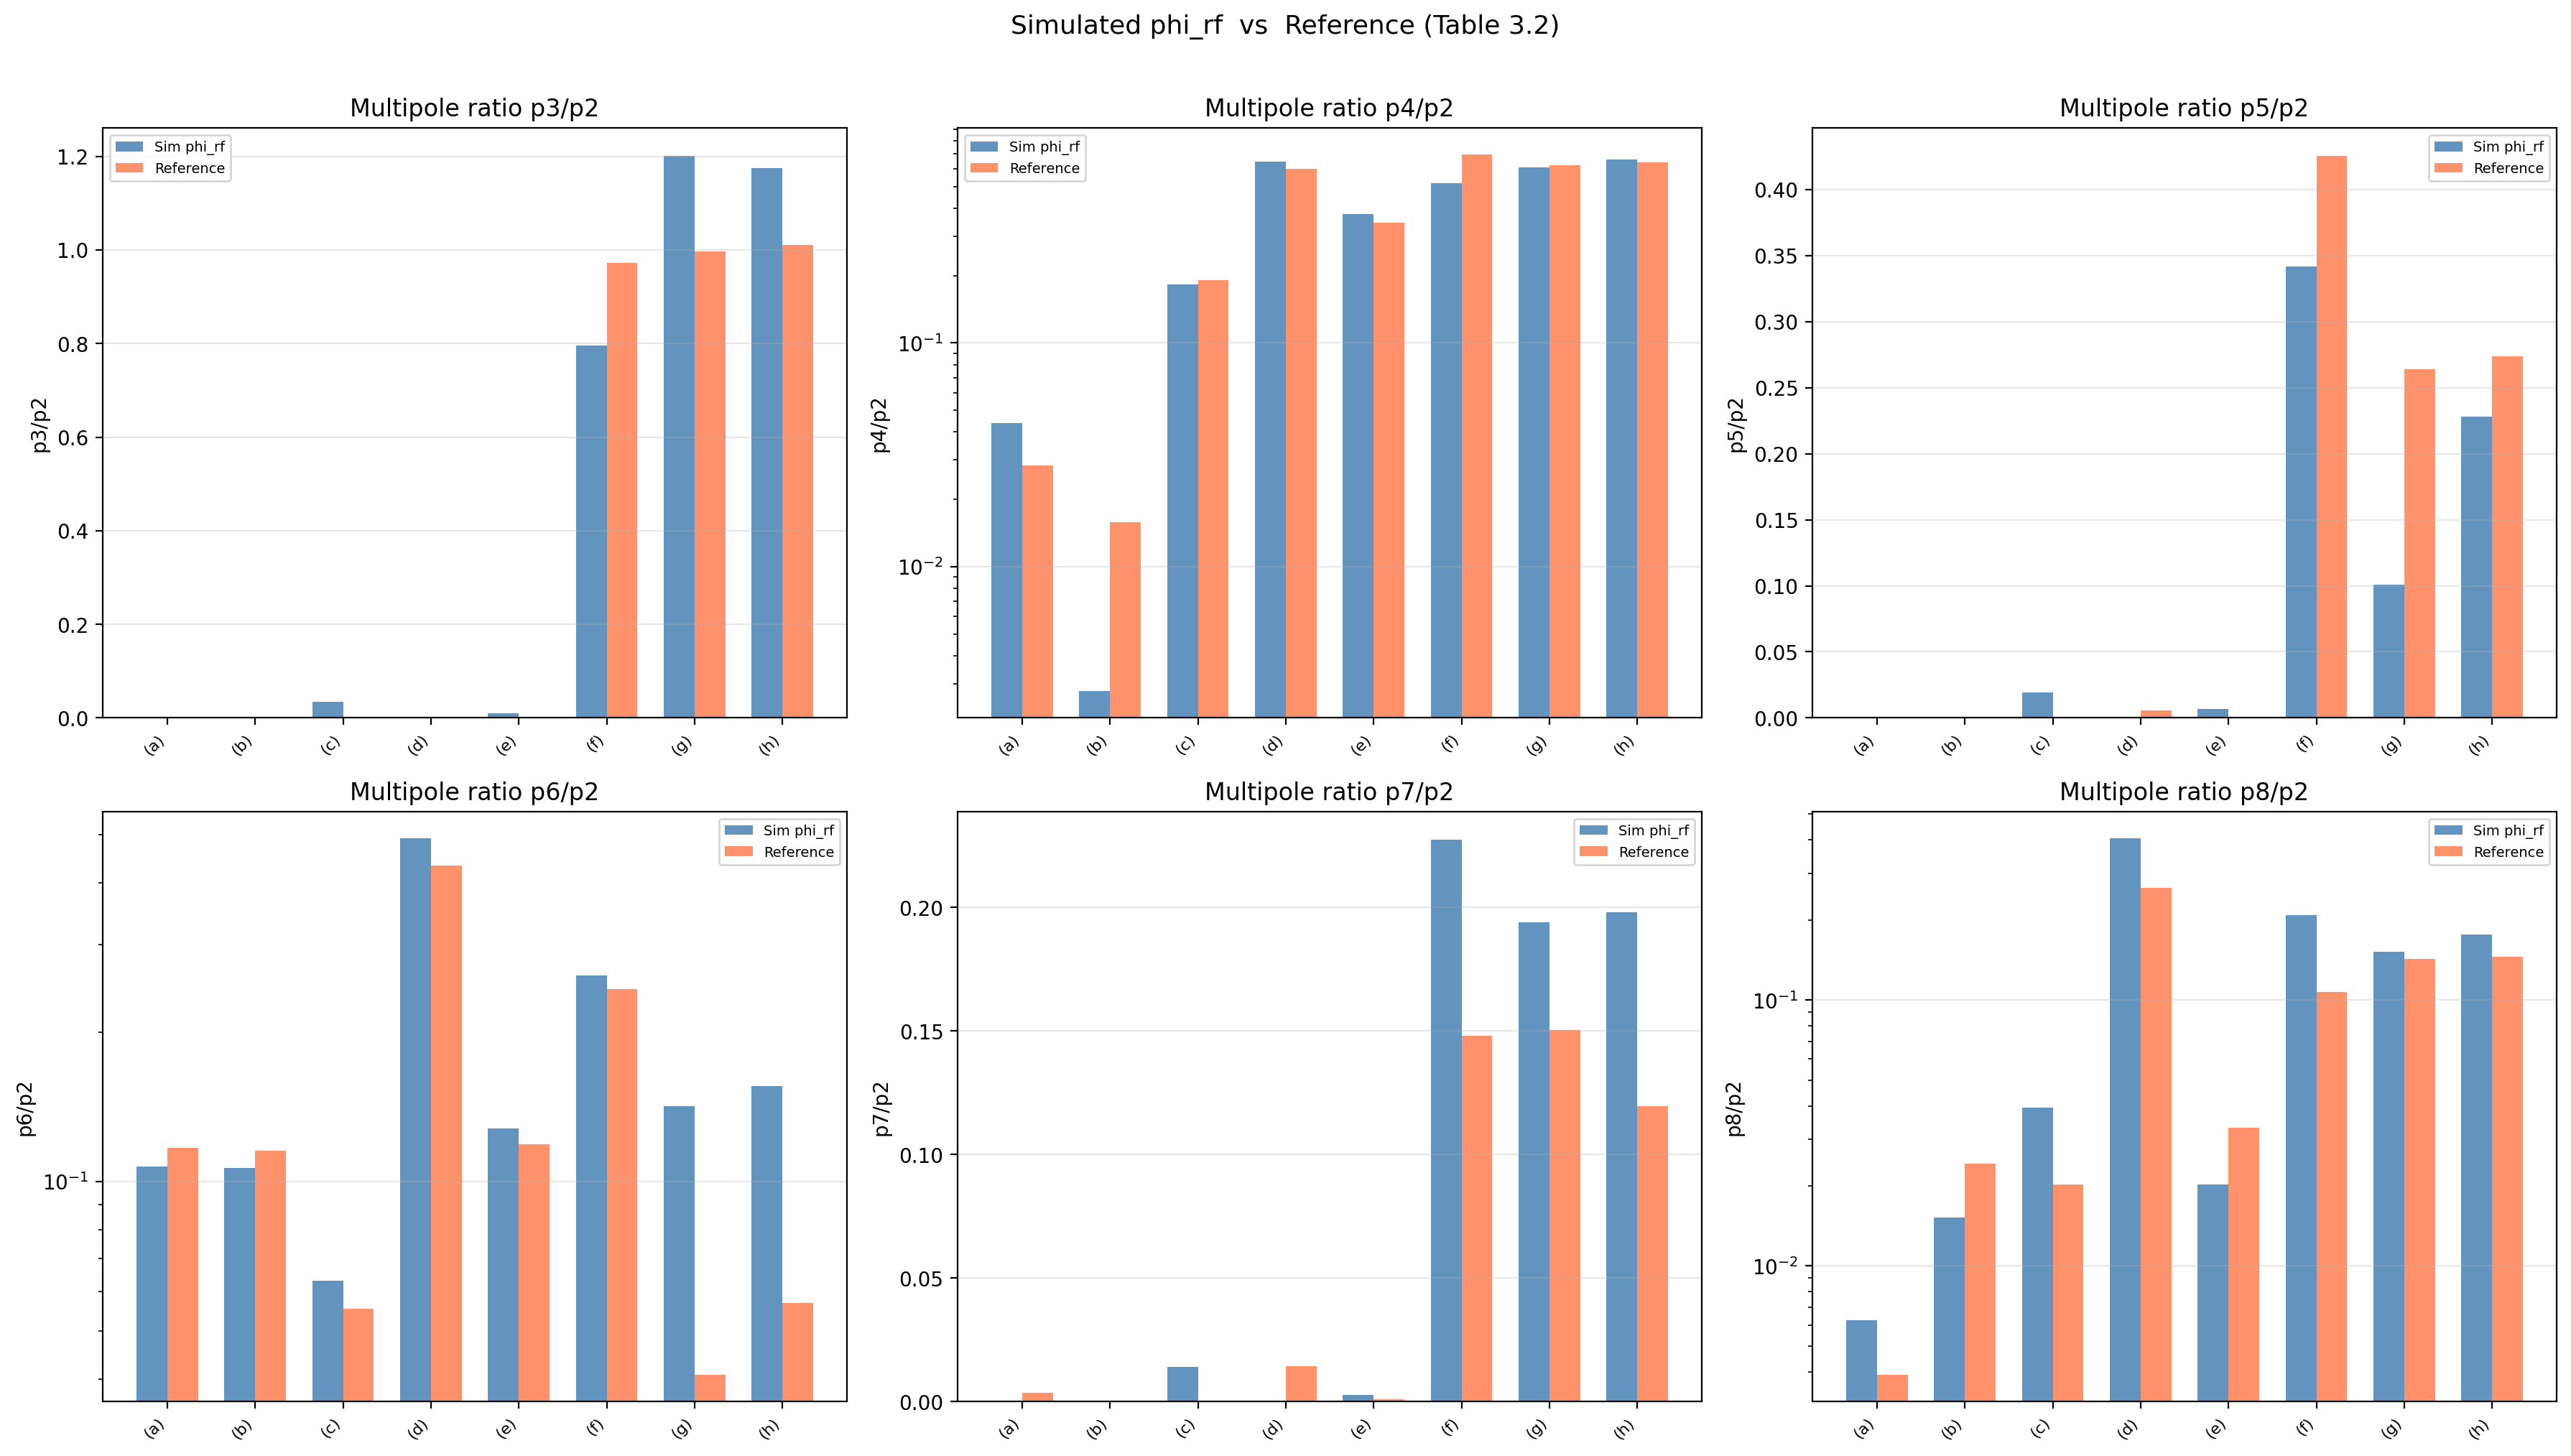
\includegraphics[width=0.9\linewidth]{pngs/multipole_comparison.png}
  \caption{Multipole comparison plot generated by the notebook for the original
  set of trap geometries.}
\end{figure}

\subsection{Solid-Angle Anharmonicity for Sketch Traps}

In addition to the 2-D finite-difference cross-section solver, the notebook
includes a gridless \textbf{3-D half-space} evaluator in
\texttt{solid\_angle\_trap.py}. This implements the surface-electrode Green's
function form
\[
  \phi(x,y,z)
  =
  \frac{z}{2\pi}
  \iint_S
  \frac{V(x',y')}{\left[(x-x')^2+(y-y')^2+z^2\right]^{3/2}}
  \,\mathrm{d}x'\,\mathrm{d}y',
\]
which, for a polygonal electrode held at voltage \(V\), reduces to
\[
  \phi_{\mathrm{electrode}}
  =
  \frac{V}{2\pi}\,\Omega_{\mathrm{polygon}},
\]
where \(\Omega\) is the solid angle subtended by the polygon as viewed from the
field point. The implementation uses the van Oosterom--Strackee edge sum on
unit vectors from the field point to each vertex.

\paragraph{Coordinate map.}
Sketch coordinates are interpreted as positions \emph{in the chip plane}
\(z=0\):
\[
  (x_{\mathrm{sketch}},y_{\mathrm{sketch}})
  \longrightarrow
  (x,y,0).
\]
The ion sits at height \(z_{\mathrm{ion}}\) above that plane, typically
\(z_{\mathrm{ion}}=30~\mu\mathrm{m}\). This differs from the FDM sketch sweep,
which places the nominal ion at \(y=30~\mu\mathrm{m}\) in the same 2-D
cross-section as the electrodes. The solid-angle path is the correct model when
all electrodes are treated as coplanar on the substrate and the ion is
\emph{above} the surface.

\paragraph{Pseudopotential and multipoles.}
At fixed \(z=z_{\mathrm{ion}}\), the code evaluates \(\phi_{\mathrm{rf}}\) on a
planar grid, forms
\[
  \Phi_{\mathrm{ps}}
  =
  \frac{q}{4m\Omega^2}
  \left(V_{\mathrm{RF}}^2|\nabla\phi_{\mathrm{rf}}|^2\right),
\]
finds the local minimum in the chip plane near \((0,0)\), subtracts
\(\Phi_{\min}\), and fits the same circular multipoles as above---centered on
the \textbf{refined null}, not the initial guess. Anharmonicity is reported as
\(p_n/p_2\) for \(n=3,\ldots,8\) on both \(\phi_{\mathrm{rf}}\) and
\(\Phi_{\mathrm{ps}}\). Optional Cartesian Taylor coefficients (e.g.\
\(c_{40}/c_{20}^2\)) are stored for intuition.

\paragraph{Outputs.}
\begin{itemize}
  \item \texttt{csv/sketch\_trap\_anharmonicity\_solid\_angle.csv}
  \item \texttt{pngs/sketch\_trap\_anharmonicity\_vs\_theta.png}
\end{itemize}
Large \(\Phi_{\mathrm{ps}}\) ratios \(p_4/p_2\), \(p_6/p_2\), etc.\ indicate
stronger deviation from an ideal quadrupole and therefore stronger
anharmonicity. The coplanar model does not include raised or trenched
electrodes out of the plane.

\begin{figure}[H]
  \centering
  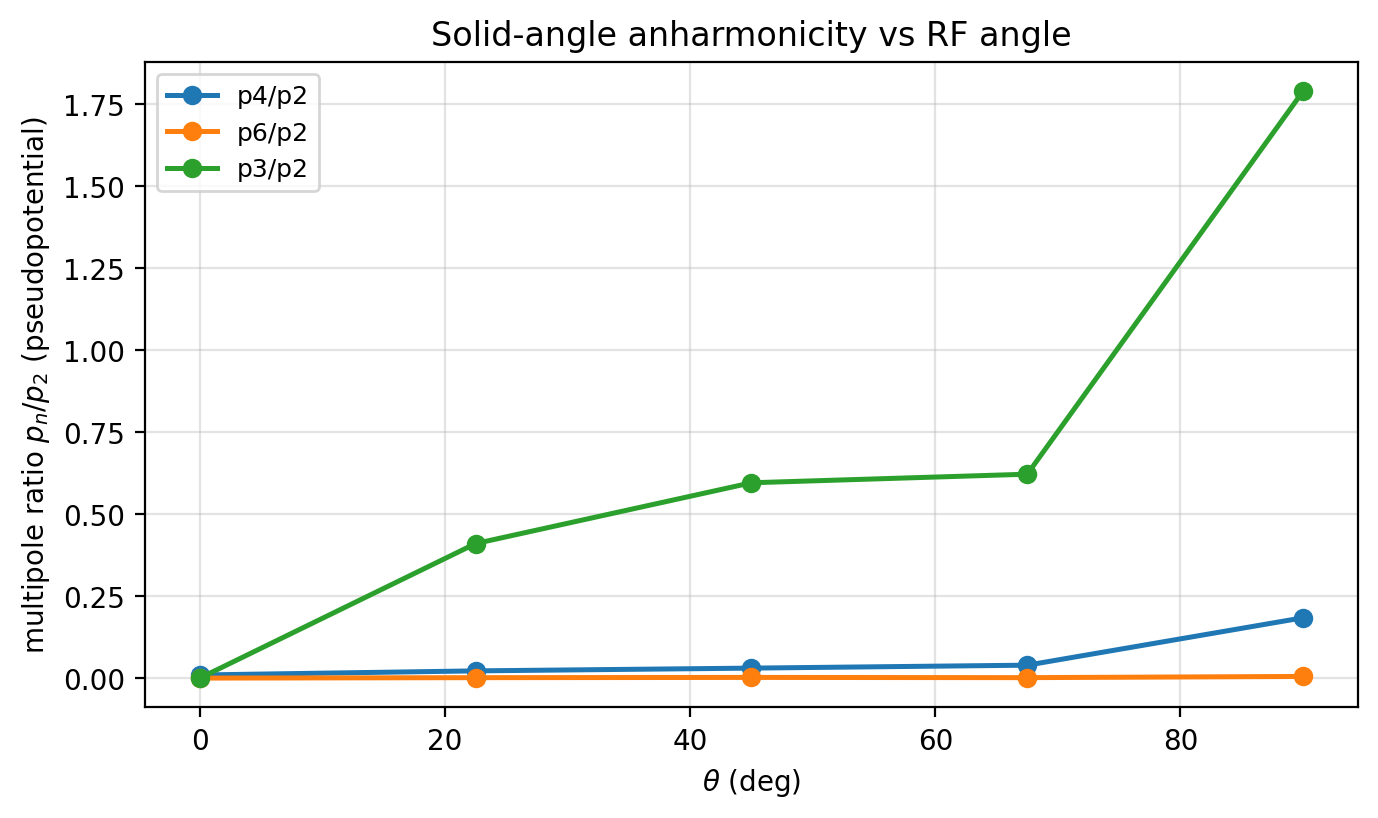
\includegraphics[width=0.82\linewidth]{pngs/sketch_trap_anharmonicity_vs_theta.png}
  \caption{Solid-angle pseudopotential multipole ratios \(p_n/p_2\) versus inner
  RF angle \(\theta\) for the five sketch geometries.}
\end{figure}

\newpage

\section{Trap Depth and Profile Plots}

The notebook uses a line cut through the shifted pseudopotential to estimate a
trap-depth scale. After finding the local pseudopotential minimum, the code
extracts a one-dimensional profile through the null. The profile is converted
to millielectron-volts by using the fact that one volt of electric potential
corresponds to one electron-volt for a singly charged ion:
\[
  \Delta E\ [\mathrm{meV}]
  =
  1000\,
  \Delta\Phi_{\mathrm{ps}}\ [\mathrm{V}].
\]

The profile is shifted so the minimum is zero. The code then looks on both
sides of the minimum and estimates the trap depth as the smaller of the two
barrier heights:
\[
  D
  =
  \min\left(
      \max_{\mathrm{left}}\Delta\Phi_{\mathrm{ps}},
      \max_{\mathrm{right}}\Delta\Phi_{\mathrm{ps}}
  \right).
\]
This conservative choice reports the shallower escape direction in the plotted
line cut. The value is stored as \texttt{profile\_depth\_mev}.

\subsection{Reference-Style Depth Summary}

For the sketch geometries, the notebook now creates a depth-summary file and
plot:
\begin{itemize}
  \item \texttt{csv/sketch\_trap\_depth\_summary.csv}
  \item \texttt{pngs/sketch\_trap\_depth\_vs\_angle\_and\_h.png}
\end{itemize}
The summary plot shows trap depth versus the RF angle \(\theta\), and also
trap depth versus nearest electrode distance \(h\). This is inspired by the
reference figure in which trap frequency or trap quality is plotted against a
geometric height parameter.

\begin{figure}[H]
  \centering
  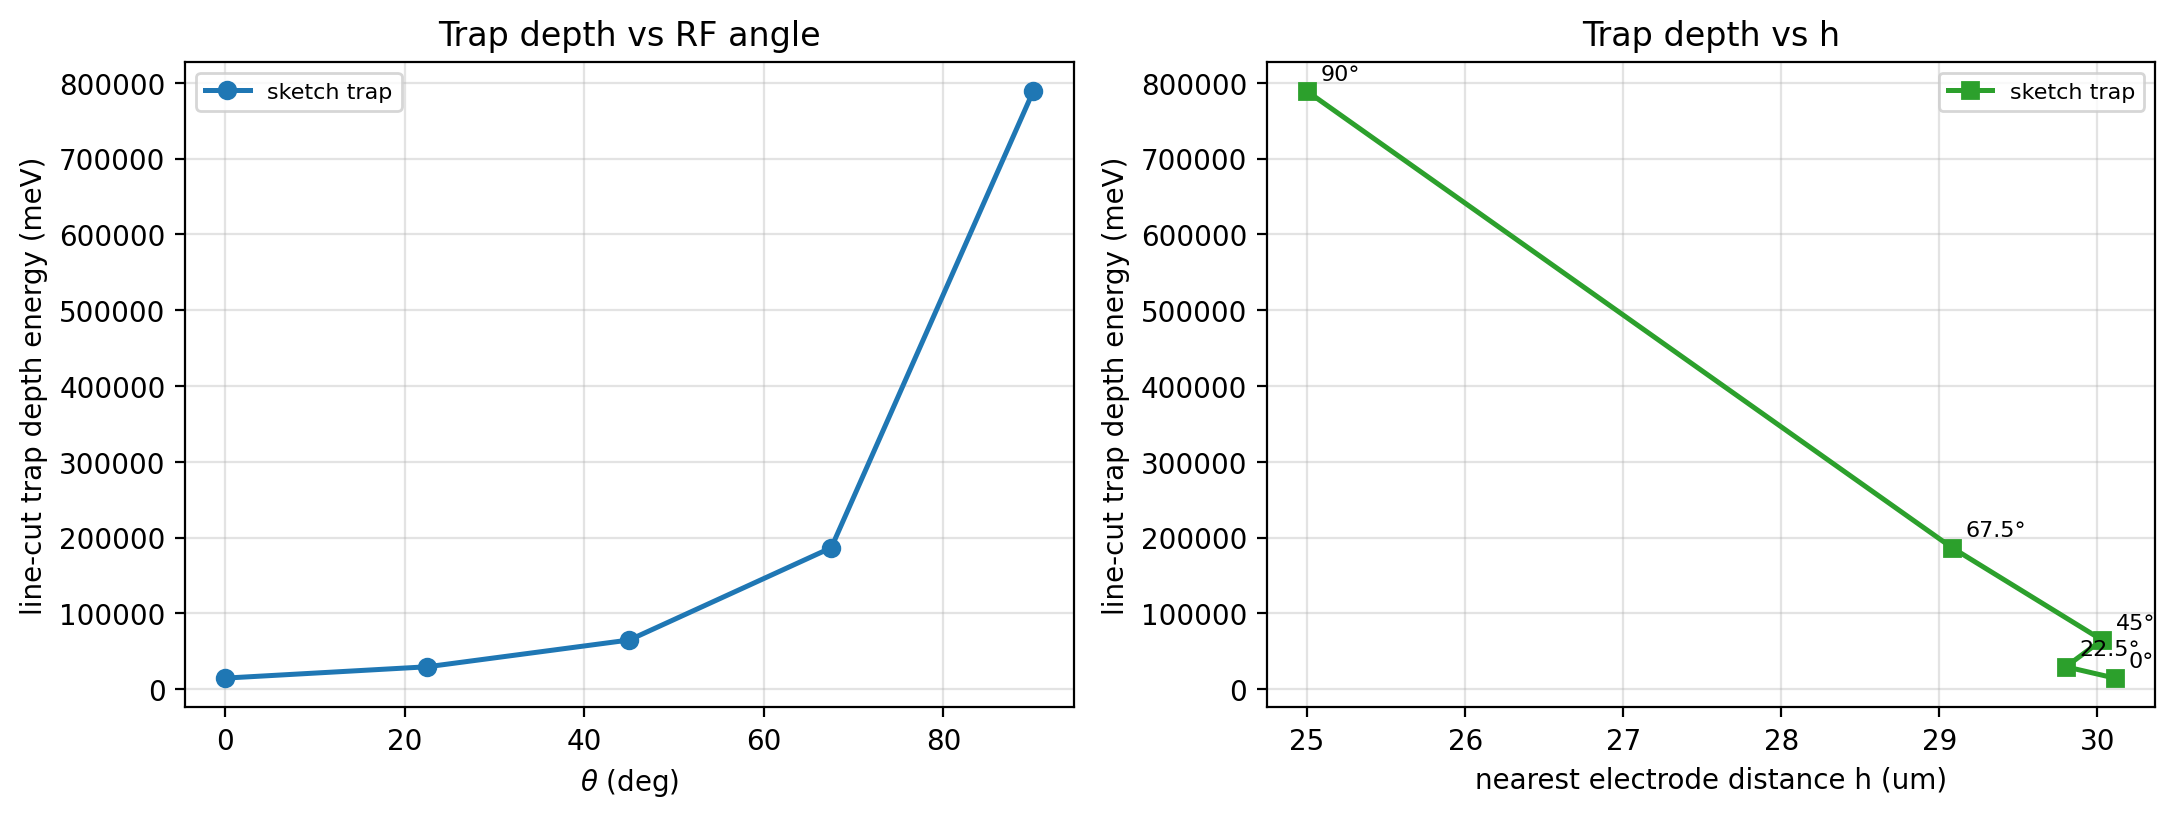
\includegraphics[width=0.9\linewidth]{pngs/sketch_trap_depth_vs_angle_and_h.png}
  \caption{Depth-summary plot for the five sketch-generated geometries. The
  first panel compares line-cut depth with RF angle. The second panel compares
  line-cut depth with the nearest-electrode distance \(h\).}
\end{figure}

\newpage

\section{How \texttt{simulate\_trap} Works}

The main driver function is \texttt{simulate\_trap(builder, name, grid,
dom\_scale, plot)}. A geometry builder is any function that returns
\[
  (\texttt{electrodes},\ \texttt{ion\_y\_guess}).
\]
The current analysis mostly fixes the nominal ion/RF-null at \((0,0)\), so
\texttt{ion\_y\_guess} is not the primary control variable.

\subsection{Pipeline}

The simulation pipeline is:
\begin{enumerate}[label=\arabic*.]
  \item Call the geometry builder to get the electrode list.
  \item Determine the computational domain size from the electrode extents.
  \item Construct a square \(N\times N\) grid.
  \item Rasterize electrode polygons/rectangles into masks.
  \item Solve the sparse Laplace problem for \(\phi_{\mathrm{rf}}\).
  \item Validate the finite-difference solution.
  \item Compute ion-electrode distance \(R\) and choose a multipole fit radius.
  \item Fit multipole amplitudes for \(\phi_{\mathrm{rf}}\).
  \item Compute the pseudopotential from \(|\nabla\phi_{\mathrm{rf}}|^2\).
  \item Search for the local pseudopotential minimum and subtract it.
  \item Fit pseudopotential multipole ratios where meaningful.
  \item Plot \(\phi_{\mathrm{rf}}\), shifted pseudopotential, and line-cut
        depth.
  \item Return a dictionary of ratios, raw coefficients, null location, depth,
        and validation data.
\end{enumerate}

\subsection{Returned Data}

The returned dictionary includes:
\begin{lstlisting}[language=Python]
{
    'rf_ratios': rf_rat,
    'ps_ratios': ps_rat,
    'rf_p': rf_p,
    'ps_p': ps_p,
    'is_surface': is_surface,
    'ps_min': ps_min,
    'rf_null': (null_x, null_y),
    'profile_depth_mev': profile_depth_mev,
    'validation': validation
}
\end{lstlisting}
These fields are later collected into comparison tables, CSV files, and summary
plots. For example, the sketch sweep stores its results in
\texttt{SKETCH\_TRAP\_DEPTH\_RESULTS}.

\subsection{Plotting}

The main plot contains two panels. The first panel shows \(\phi_{\mathrm{rf}}\)
with a diverging colormap. The second panel shows the shifted pseudopotential
near the local RF null using a clipped \texttt{viridis} scale so the low-energy
structure is visible. A separate profile plot shows the line-cut depth in
millielectron-volts.

\newpage

\section{Validation and Numerical Checks}

The notebook contains a finite-difference validation suite with tolerance
\[
  \texttt{PHYSICS\_TOL} = 10^{-3}.
\]
The function \texttt{validate\_physics\_fd} combines two checks.

\subsection{Laplace Residual Check}

The function \texttt{check\_laplace\_fd} recomputes the finite-difference
Laplacian of the solved potential in vacuum pixels. It reports both:
\begin{itemize}
  \item an all-vacuum residual, and
  \item a bulk residual that excludes pixels near electrode boundaries.
\end{itemize}
The bulk check is usually the more meaningful one because rasterized polygon
edges create stair-step boundaries. Near those boundaries, local finite-
difference residuals can be dominated by mask geometry rather than by the
quality of the sparse solve.

\subsection{Electrode Voltage Check}

The function \texttt{check\_electrode\_voltage\_fd} verifies that every
electrode mask pixel in the solved grid has the prescribed voltage. This catches
geometry mistakes where two electrodes with different voltages overlap on the
same grid. Such overlap is not physically meaningful in a Dirichlet
finite-difference solve because a single pixel cannot be both \(+1\) and
\(-1\) at the same time.

This check was especially useful for the sketch-based trap generator. The
visual geometry intentionally places RF pads using the exact endpoint of an
angled RF segment. For solver masks, however, touching different-voltage
electrodes can share grid pixels at high angles. The notebook therefore allows
a small solver-only contact gap while preserving the endpoint-based visual
construction.

\subsection{Interpreting PASS and FAIL}

A typical validation printout contains:
\begin{lstlisting}
Physics validation (tol=1.0e-03):
  Laplace (all vacuum)      : PASS
  Laplace (bulk, >3px gap)  : PASS
  Electrode grid voltage    : PASS
\end{lstlisting}
If the electrode-voltage check fails, the most common cause is overlapping
electrode masks. If the Laplace residual fails only at boundary-adjacent pixels
but passes in the bulk, the solution may still be usable, but the geometry mask
or grid resolution should be inspected.

\newpage

\section{The Sketch Trap Sweep}

The sketch-based sweep is the newest part of the notebook. It is organized in
two stages:
\begin{enumerate}[label=\arabic*.]
  \item Generate clean geometry plots and masks directly from the sketch
        construction.
  \item Translate each geometry below the nominal ion position and run the
        full \texttt{simulate\_trap} pipeline.
\end{enumerate}

\subsection{Geometry Stage}

The generator uses:
\begin{itemize}
  \item ground length \(50\ \mu\mathrm{m}\),
  \item ground thickness \(4\ \mu\mathrm{m}\),
  \item RF thickness \(4\ \mu\mathrm{m}\),
  \item inner angled RF length \(50\ \mu\mathrm{m}\),
  \item outer RF pad length \(50\ \mu\mathrm{m}\),
  \item ground-to-RF gap \(2\ \mu\mathrm{m}\).
\end{itemize}
For each angle, the central ground is horizontal and centered at \(x=0\).
The right inner RF segment leaves the right ground end at angle \(\theta\);
the left inner RF segment leaves the left ground end at angle
\(180^\circ-\theta\). The trap remains symmetric about \(x=0\).

\subsection{Simulation Stage}

The function \texttt{make\_sketch\_trap\_sim\_builder} translates the generated
geometry downward so that the top of the electrode structure is a chosen
distance below the ion. The default is
\[
  h_{\mathrm{ion}} = 40\ \mu\mathrm{m}.
\]
The full sweep function,
\texttt{run\_sketch\_trap\_simulation\_sweep}, runs:
\[
  \theta = 0^\circ,\ 22.5^\circ,\ 45^\circ,\ 67.5^\circ,\ 90^\circ.
\]
It saves main and profile plots using filenames of the form
\[
  \texttt{pngs/sketch\_trap\_sim\_theta\_...\_main.png}
\]
and
\[
  \texttt{pngs/sketch\_trap\_sim\_theta\_...\_profile.png}.
\]

\begin{figure}[H]
  \centering
  \begin{subfigure}{0.48\linewidth}
    \centering
    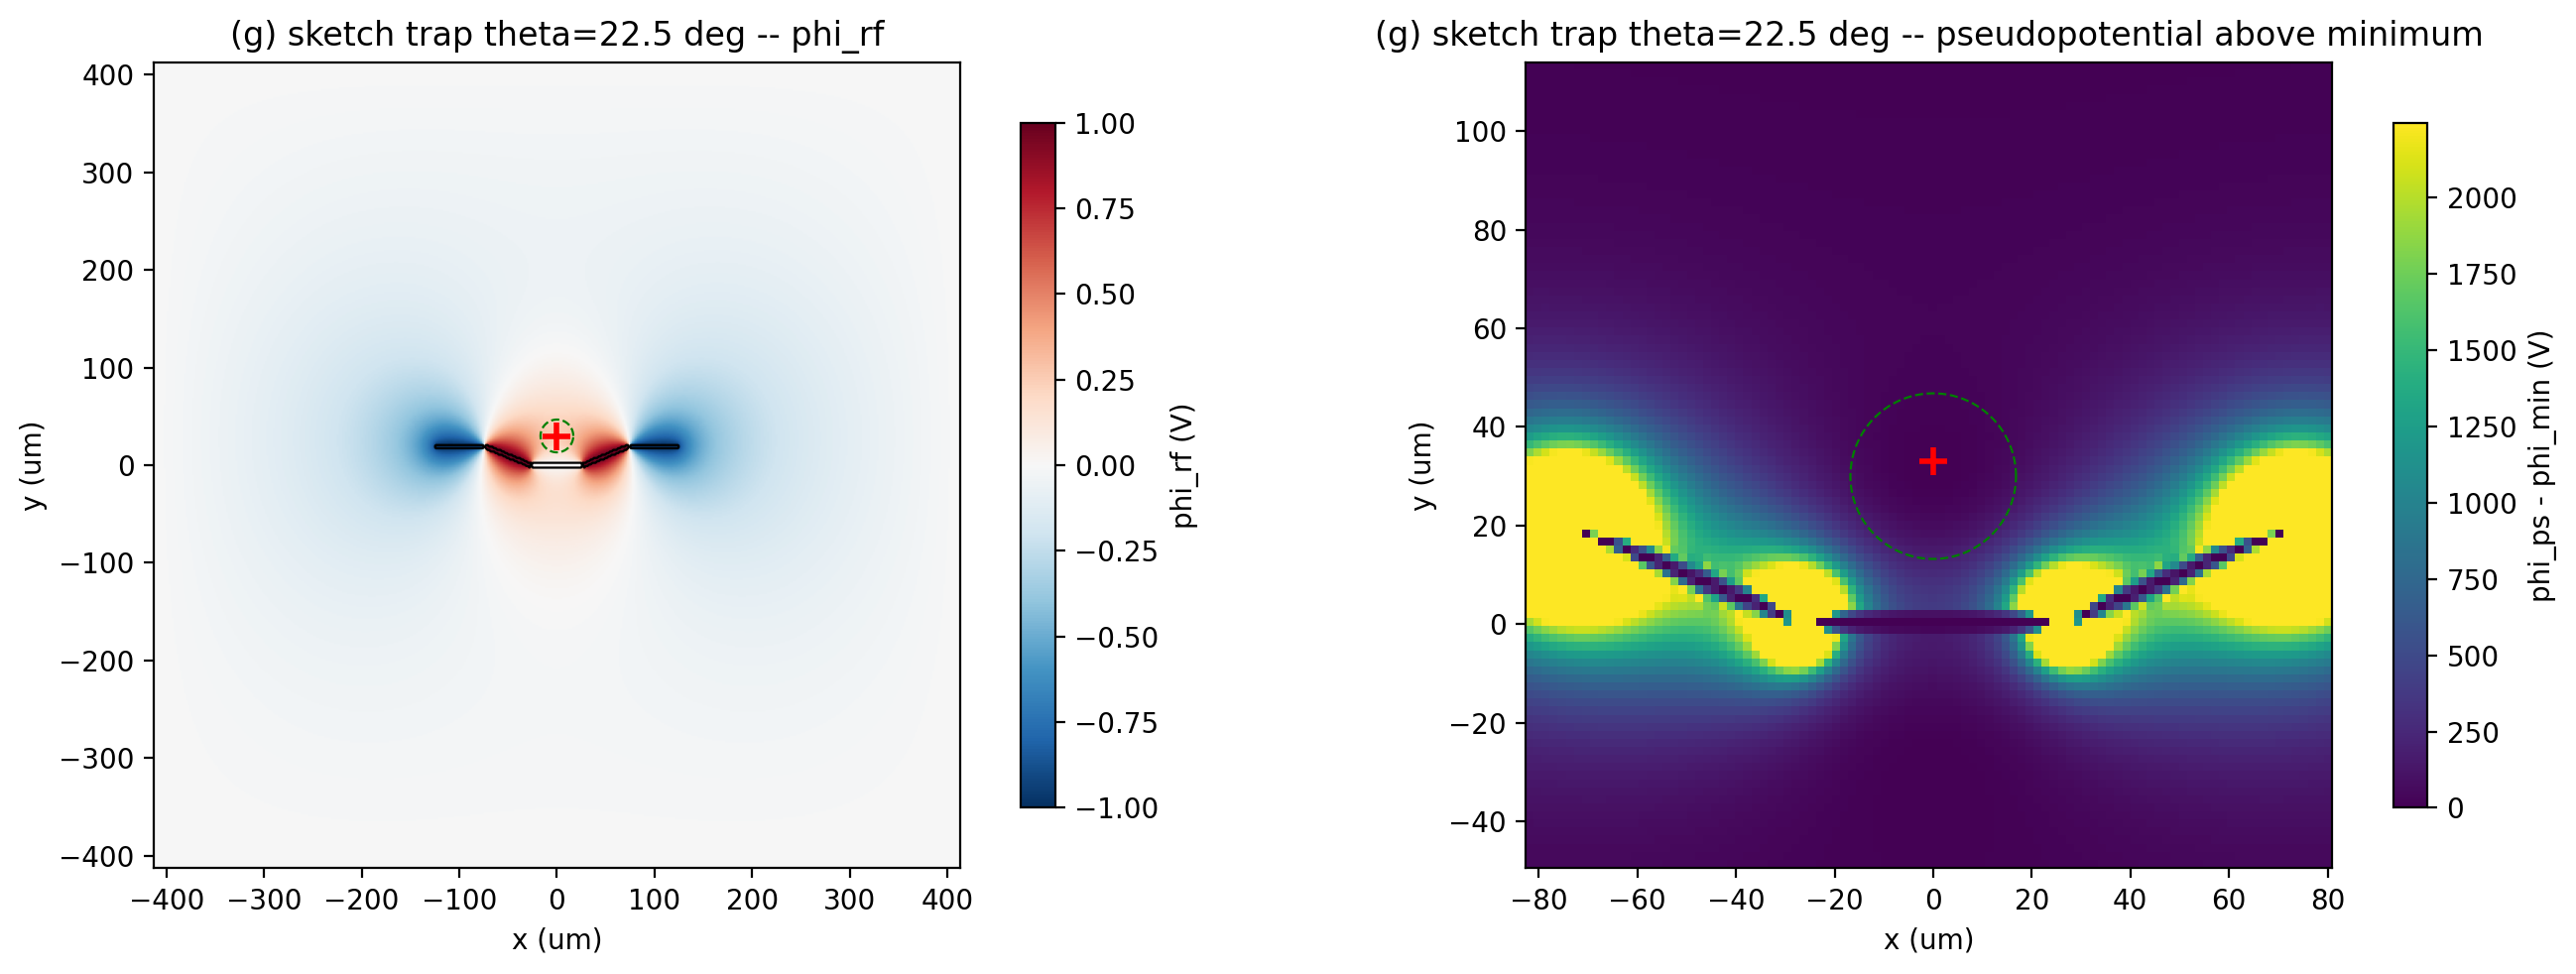
\includegraphics[width=\linewidth]{pngs/sketch_trap_sim_theta_22p5deg_main.png}
    \caption{\(\theta=22.5^\circ\) main plot.}
  \end{subfigure}
  \hfill
  \begin{subfigure}{0.38\linewidth}
    \centering
    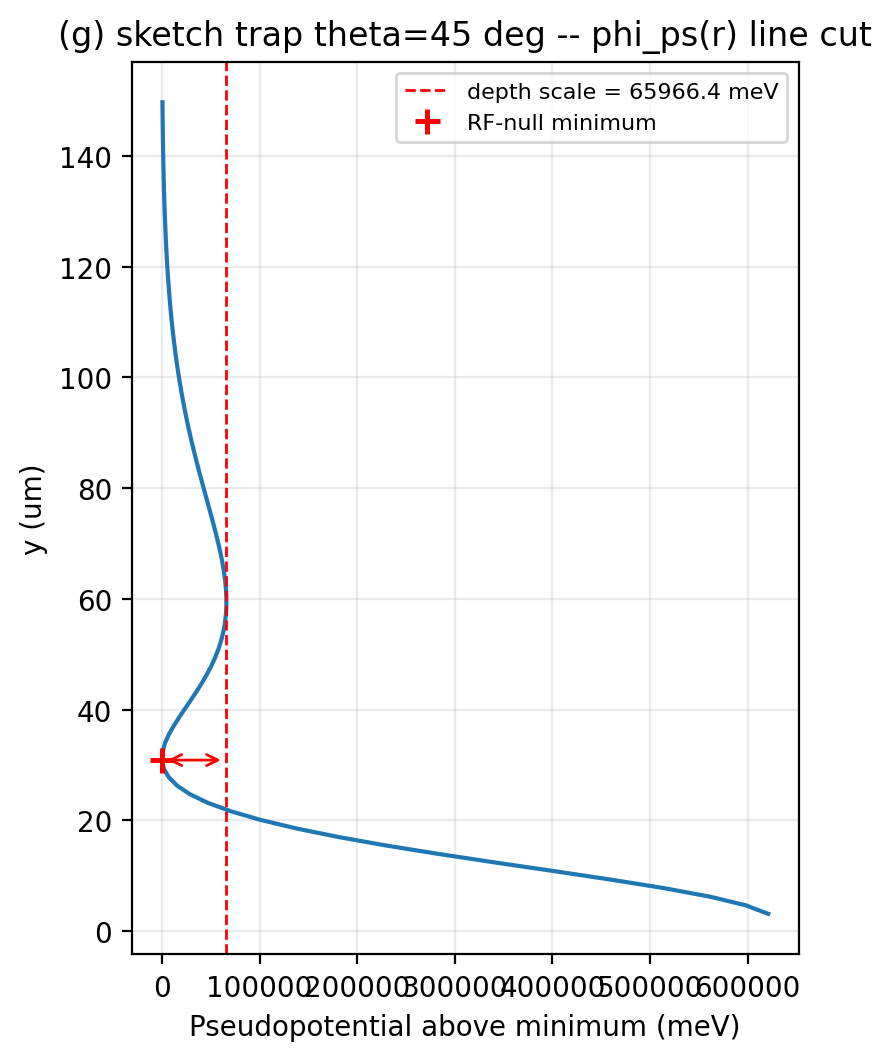
\includegraphics[width=\linewidth]{pngs/sketch_trap_sim_theta_45p0deg_profile.png}
    \caption{\(\theta=45^\circ\) profile plot.}
  \end{subfigure}
  \caption{Examples of the same plot types produced for the original traps
  (a)--(h), now applied to the sketch-generated geometries.}
\end{figure}

\newpage

\section{Important Assumptions and Limitations}

\subsection{Two-Dimensional Approximation}

The notebook solves a two-dimensional Laplace problem. This is useful for
cross-section design, but real ion traps are three-dimensional. End effects,
segmentation, axial confinement, loading slots, finite electrode thickness,
dielectrics, and package geometry can all change the actual field. The 2D
calculation should therefore be interpreted as a design-screening tool rather
than a final engineering model.

\subsection{Ideal Conductors and Sharp Boundaries}

Electrodes are treated as ideal Dirichlet conductors with perfectly sharp
boundaries. The masks approximate polygon boundaries on a Cartesian grid. This
means high curvature, narrow gaps, and touching corners can be sensitive to
grid resolution.

\subsection{Pseudopotential Approximation}

The pseudopotential approximation assumes the RF drive is fast enough that the
ion's micromotion can be averaged over one RF cycle. It also assumes the ion
motion remains in a region where the secular approximation is valid. Near very
large fields, sharp barriers, or unstable Mathieu parameters, a full
time-dependent trajectory calculation would be more accurate.

\subsection{Trap Depth from a One-Dimensional Cut}

The profile depth is a line-cut estimate. It is useful for comparing similar
geometries, but a true trap depth is a two-dimensional or three-dimensional
saddle-point problem. The line cut may miss an easier escape path in another
direction. A more complete version would locate saddle points of
\(\Phi_{\mathrm{ps}}(x,y)\) in the full open domain.

\subsection{Sensitivity to the RF Null Search}

For some geometries, especially asymmetric or highly angled designs, the local
pseudopotential minimum can shift away from the nominal origin. The code
searches near the nominal ion position, subtracts the local minimum, and then
uses that shifted potential for plotting. If a geometry creates multiple local
minima, the search region and edge margin should be reviewed.

\newpage

\section{How to Read and Extend the Notebook}

The notebook is easiest to understand as a layered workflow:
\begin{enumerate}[label=\arabic*.]
  \item Constants and imports define the physical ion and RF drive.
  \item Core solver functions define masks, sparse Laplace solving,
        pseudopotential conversion, multipole fitting, and ion-electrode
        distance calculations.
  \item Geometry builders define electrode polygons and voltages.
  \item \texttt{simulate\_trap} runs one complete physics calculation.
  \item Sweep cells call \texttt{simulate\_trap} repeatedly and save figures.
  \item Summary cells collect CSVs and comparison plots.
\end{enumerate}

\subsection{Adding a New Geometry}

To add a new trap, write a builder function:
\begin{lstlisting}[language=Python]
def trap_new_geometry():
    electrodes = [
        {'cx': ..., 'cy': ..., 'w': ..., 'h': ..., 'V': 1.0, 'label': 'RF'},
        {'cx': ..., 'cy': ..., 'w': ..., 'h': ..., 'V': 0.0, 'label': 'GND'},
    ]
    return electrodes, 0.0
\end{lstlisting}
For tilted electrodes, include a \texttt{poly} key. Then run:
\begin{lstlisting}[language=Python]
result = simulate_trap(trap_new_geometry, '(new) candidate trap',
                       grid=501, dom_scale=1.0, plot=True)
\end{lstlisting}

\subsection{Increasing Accuracy}

The most direct way to increase spatial accuracy is to increase the grid size,
for example from \(501\times501\) to \(1001\times1001\) or \(2001\times2001\).
This improves boundary resolution but makes the sparse solve much slower and
more memory-intensive. A good workflow is:
\begin{enumerate}[label=\arabic*.]
  \item Develop geometry at \(251\) or \(501\) grid points.
  \item Check validation passes.
  \item Run selected final geometries at higher resolution.
  \item Compare whether the RF null, multipole ratios, and depth estimates are
        stable.
\end{enumerate}

\subsection{Improving Trap Depth Estimates}

A future improvement would compute the trap depth by searching the full 2D
open region for saddle points. That could be done by:
\begin{itemize}
  \item locating all local minima of \(\Phi_{\mathrm{ps}}\);
  \item building contours around the chosen trapping minimum;
  \item finding the lowest contour that connects to the domain boundary or an
        electrode; and
  \item reporting that contour height as the 2D escape barrier.
\end{itemize}

\section{Summary}

\texttt{multipole\_table\_replication.ipynb} implements a complete 2D RF
ion-trap modeling workflow. It converts electrode layouts into masks, solves
Laplace's equation with Dirichlet boundary conditions, computes the RF
pseudopotential from the squared electric-field amplitude, fits multipole
ratios using circular Fourier analysis, validates the numerical solution, and
produces comparison plots and CSV summaries. The physics is based on the
standard ponderomotive pseudopotential
\[
  \Phi_{\mathrm{ps}}
  =
  \frac{q}{4m\Omega^2}
  V_{\mathrm{RF}}^2|\nabla\phi_{\mathrm{rf}}|^2,
\]
with \({}^{9}\mathrm{Be}^{+}\), \(V_{\mathrm{RF}}=500\ \mathrm{V}\), and
\(\Omega/2\pi=30\ \mathrm{MHz}\). The code is modular: new geometries can be
added by writing builder functions that return electrode dictionaries. The
sketch-based generator extends this workflow by constructing angle-dependent
surface-electrode layouts directly from geometric endpoints and then applying
the same solver and plotting pipeline used for traps (a)--(h).

\end{document}
